\documentclass[
    11pt,
    a4paper,
    egregdoesnotlikesansseriftitles,
    toc=chapterentrywithdots,
    twoside,openright,
    titlepage,
    parskip=half,
    headings=normal,  % reduces heading size
    listof=totoc,
    bibliography=totoc,
    index=totoc,
    captions=tableheading,  % caption below table
    chapterprefix,
    listof=flat,
    final
]{scrbook}


\newcommand{\mailto}[1]{\href{mailto:#1}{#1}}
\newcommand*{\signatureAndDate}[1]{%
	\\[0.05cm]
	\par\noindent\makebox[10cm]{\hrulefill} \makebox[5.0cm]{\hrulefill}%
	\par\noindent\makebox[10cm][l]{#1}      \makebox[5.0cm][l]{Datum}%
}%

\newcommand{\quickFig}[3]{\begin{figure}[htbp]\centering\includegraphics[width=1\linewidth]{#1}\caption{#2}\label{fig:#3}\end{figure}}

%\addto\captionsenglish{\renewcommand{\chaptername}{}} % use this to change "Chapter" to sth else
%\addto\captionsngerman{\renewcommand{\chaptername}{}} % same for german thesis
 
% custom head and foot
\usepackage[automark]{scrlayer-scrpage}
\pagestyle{scrheadings}
%\ihead{\headmark}
\chead{}
%\ohead{\pagemark}
\renewcommand*\chaptermarkformat{\chapappifchapterprefix{\ }% 
	\thechapter.\enskip}

\RedeclareSectionCommand[tocindent=0pt]{section}
\RedeclareSectionCommand[tocindent=0pt]{subsection}
%\RedeclareSectionCommand[tocnumwidth=70pt]{chapter}


% other packages
\usepackage{minted}
\usepackage[utf8]{inputenc}
\usepackage[T1]{fontenc}
\usepackage{lmodern,relsize,textcomp,csquotes}
\usepackage{amsmath,amsfonts}
% \usepackage[ngerman, english]{babel}  % English thesis
\usepackage[english, ngerman]{babel}  % German thesis
\usepackage[final]{graphicx}
\usepackage{setspace,geometry,xcolor}
\usepackage{makeidx}
\usepackage{paralist,ifthen,todonotes}
\usepackage{url}
\usepackage[toc]{glossaries}
\usepackage{pdfpages}
\usepackage{xcolor}
\usepackage{varioref}
\usepackage{tcolorbox}
\usepackage{caption}
\usepackage{subcaption}
\tcbuselibrary{minted,skins,breakable,listings}

% table setup
\usepackage{rotating}
\usepackage{longtable}
\usepackage{array}
\usepackage{ragged2e}
\usepackage{lscape}\usepackage[
	backend=biber, 
	natbib=true,
	style=numeric,
	sorting=none
]{biblatex}


% pdf hyperref
\usepackage[
bookmarks=true,
bookmarksopen=true,
bookmarksnumbered=true,
bookmarksopenlevel=1,
pdftitle={\titel},
pdfauthor={\autor},
pdfcreator={\autor},
pdfsubject={\titel},
pdfpagelabels=true,
colorlinks=true,
linkcolor=red,
urlcolor=magenta,
anchorcolor=black,
citecolor=cyan,
filecolor=magenta,
menucolor=red,
plainpages=false,
hypertexnames=true,
linktocpage=true,
]{hyperref}
\usepackage[inkscapeformat=png]{svg}

\usepackage[ngerman]{cleveref}
\usepackage{scrhack}

% configure your listings style
\usepackage{listings}


\lstset{
	tabsize=3,
	extendedchars=true,
	frame=single,
	showstringspaces=true,
	numbers=left,
	numberstyle=\small,
	breakautoindent=true
}

% page setup
% \setlength{\topskip}{\ht\strutbox}
\geometry{paper=a4paper,left=2.5cm,top=3.0cm,bindingoffset=.8cm}
\onehalfspacing
\frenchspacing
\clubpenalty = 10000
\widowpenalty = 10000 
\displaywidowpenalty = 10000


% this sets the color and font for the minted linenumber
\renewcommand{\theFancyVerbLine}{\sffamily
	\textcolor[rgb]{0.6,0.05,0.05}{\scriptsize
		\oldstylenums{\arabic{FancyVerbLine}}}}


\newlength\myboxwidth
\setlength{\myboxwidth}{\dimexpr\textwidth-20\fboxsep}

\newtcolorbox[auto counter,
crefname={Pseudocodeblock}{Pseudocodeblöcke}]%
{pseudoCodeblock}[1]{
	arc=1mm, 
	breakable,
	left=.8cm,
	colback=white,
	coltitle=black,
	colframe=blue!40!white,
	fonttitle=\sffamily,
	label=#1,
	title=Pseudocode \thetcbcounter, 
}
\newenvironment{pseudoCode}[5]{\VerbatimEnvironment\begin{pseudoCodeblock}{#5}\colorbox{blue!40!white}{\textbf{#1}(#2)}\\#3\begin{minted}[linenos,breaklines,escapeinside=||,mathescape=true,firstnumber=#4,baselinestretch=1.2,tabsize=3]{python}}{\end{minted}\end{pseudoCodeblock}}


\newtcolorbox[auto counter,
crefname={Rust Block}{Rust Blöcke}]%
{rustCodeblock}[1]{
	arc=0mm, 
	breakable,
	left=.8cm,
	colback=white,
	coltitle=black,
	colframe=red!40!white,
	fonttitle=\sffamily,
	label=rust:#1,
	title=Rust \thetcbcounter, 
}


\newenvironment{rustCode}[2]{\VerbatimEnvironment\begin{rustCodeblock}{#2}\begin{minted}[linenos,breaklines,firstnumber=#1,baselinestretch=1.2,tabsize=3]{rust}}{\end{minted}\end{rustCodeblock}}


\newtcolorbox[auto counter,
crefname={Python Block}{Python Blöcke}]%
{pythonCodeblock}[1]{
	arc=0mm, 
	breakable,
	left=.8cm,
	colback=white,
	coltitle=black,
	colframe=green!40!white,
	fonttitle=\sffamily,
	label=python:#1,
	title=Python \thetcbcounter, 
}


\newenvironment{pythonCode}[2]{\VerbatimEnvironment\begin{pythonCodeblock}{#2}\begin{minted}[linenos,breaklines,firstnumber=#1,baselinestretch=1.2,tabsize=3]{python}}{\end{minted}\end{pythonCodeblock}}


% TODO remove if not needed...
\usepackage{blindtext}

% load glossary entries
\makenoidxglossaries
\loadglsentries{glossary}

\begin{document}
	
	\setcounter{secnumdepth}{3}  % numerate subsections
	\setcounter{tocdepth}{2}  % ...but don't include them in toc
	
	\frontmatter
	\thispagestyle{empty}
\pdfbookmark[1]{Cover}{cov}
\begin{titlepage}

\begin{center}


\includegraphics[width=\linewidth]{figures/TH-Nuernberg-RGB.png}\\[1cm]
\LARGE{Angewandte Mathematik und Physik}\\[2cm]

\huge
\textbf{\titel}\\[1cm]
%
\Large
\artderarbeit~im Studiengang \studiengang\\[1cm]
%
\large
vorgelegt von

\Large
\autor\\[0.5cm]
\small
Matrikelnummer \matrikelnr\\[2cm]

\vspace*{\fill}

\large
\begin{tabular}{p{3cm}p{8cm}}\\
Erstgutachter:  & \quad \erstgutachter\\[1.2ex]
Zweitgutachter: & \quad \zweitgutachter\\[1.2ex]
%discomment "Betreuer" and "Unternehmen" for a thesis in a company
%Betreuer: & \quad \betreuer\\
%Unternehmen: & \quad \unternehmen
\end{tabular}
\end{center}

\begin{center}
\copyright\,\the\year
\end{center}

\vspace{-0.5cm}
\singlespacing
\small
\noindent Dieses Werk einschließlich seiner Teile ist \textbf{urheberrechtlich geschützt}.
Jede Verwertung außerhalb der engen Grenzen des Urheberrechtgesetzes ist ohne Zustimmung des Autors unzulässig und strafbar.
Das gilt insbesondere für Vervielfältigungen, Übersetzungen, Mikroverfilmungen sowie die Einspeicherung und Verarbeitung in elektronischen Systemen.

\end{titlepage}
\cleardoublepage
	
	% download the following form and complete it (hit save in your editor)
	% https://intern.ohmportal.de/fileadmin/Gelenkte_Doks/Abt/SZS/SB/SB_0050_FO_Pruefungsrechtliche_Erklaerung_und_Erklaerung_zur_Veroeffentlichung_der_Abschlussarbeit_public.pdf
	% 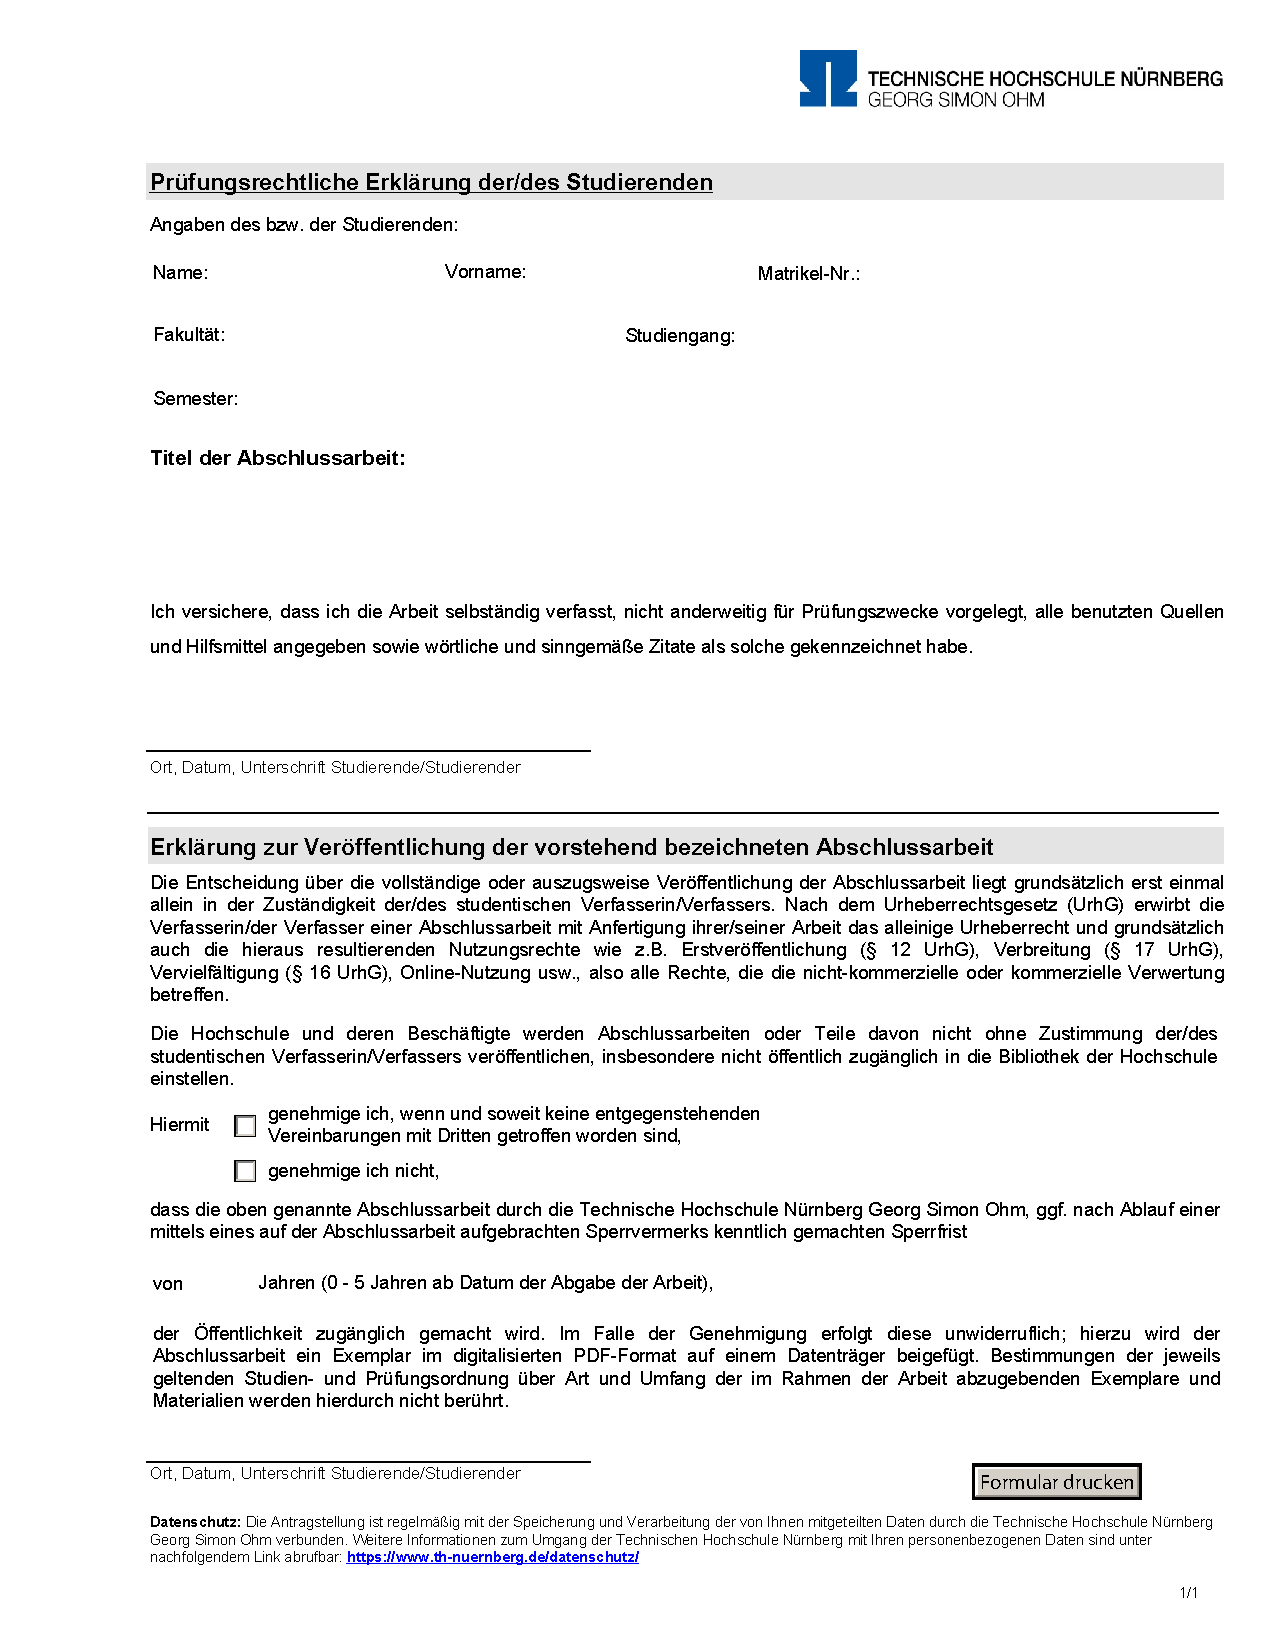
\includepdf{SB_0050_FO_Pruefungsrechtliche_Erklaerung_und_Erklaerung_zur_Veroeffentlichung_der_Abschlussarbeit_public.pdf}\cleardoublepage
	\include{content/0_abstract}\cleardoublepage
	
	\tableofcontents
	
	\mainmatter
	\begin{pythonCode}{123}{pythontest}
for i in range(10):
	print(i)
	\end{pythonCode}
\cref{python:pythontest}
	\begin{rustCode}{1}{test}
fn test(test: &mut u8) -> &mut u8{
	test
}
	\end{rustCode}
	\cref{rust:test}
	\begin{pseudoCode}
		{MASS}
		{\emph{Q}, \emph{T}}
		{\underline{Input}: \emph{Abfrageteilsequenz Q, gesamte Zeitreihe T}\\\underline{Output}: \emph{Distanzprofil D der Abfrageteilsequenz Q}}
		{11}
		{MASS}
|$m$| = Length(|$\mathbf{T}$|) - Length(|$\mathbf{P}$|)
|$\boldsymbol{\mu}, \boldsymbol{\sigma}$| = ComputeMeanStd(|$\mathbf{T}, m$|) 
|$motif\_distances, motif\_indices, motif\_subspaces, motif\_mdls$| = |$[\ ]$|
if not set otherwise
compute default values

|$candidate\_idx$| = get indices of row-wise minima in |$\mathbf{P}$|
|$nn\_idx$| = length |$d$| zero array
for k from 1 to |$d$|
|$nn\_idx[k]$| = |$\mathbf{I}[k, candidate\_idx]$|
while Length(|$motif\_distances$|) < |$max\_motifs$|
|$mdls, subspaces$| = mdl(|$\mathbf{T}, m, candidate\_idx, nn\_idx, include$|)
if k is None
|$k$| = get index of minimum in |$mdls$|
|$subspace\_k$| = |$subspaces[k]$|
|$motif\_idx$ = $candidate\_idx[k]$|
|$motiv\_value$ = $\mathbf{P}[k, motif\_idx]$|	
if (|$motif\_value > cutoffs[k]$| or |$motif\_value$| is inf
or |$motif\_value > max\_distance$|)
break	
|$query\_matches$| = match(
|$\mathbf{T}[subspace\_k, motif\_idx : motif\_idx + m]$|, |$\mathbf{T}[subspace\_k]$|,
|$\boldsymbol{\mu}[subspace\_k]$|, |$\boldsymbol{\sigma}[subspace\_k]$|, |$max\_matches$|, |$max\_distance$|,
|$atol$|, |$motif\_idx$|, |$normalize$|, |$p$|
)
if Length(|$query\_matches > min\_neighbors$|)
append |$query\_matches, subspace\_k, mdls$| to output
for idx in |$query\_matches[:, 1]$|
ApplyExclusionZone(|$\mathbf{P}, idx$|)
find new |$candidate\_idx$| and |$nn\_idx$|
return |$motif\_distances, motif\_indices, motif\_subspaces, motif\_mdls$|










asdf





	\end{pseudoCode}
	\cref{MASS}

	\chapter{Data}\label{ch:data}

\Blindtext


\begin{definitionsBlock}{test}
Definition!
\end{definitionsBlock}
\cref{def:test}
	\chapter{Method}\label{ch:method}

In this chapter, we're actually using some code!

\begin{lstlisting}[language=Python,caption={This is an example of inline listing},captionpos=b]
x = 1
if x == 1:
    # indented four spaces
    print("x is 1.")

\end{lstlisting}

You can also include listings from a file directly\cite{Goodliffe2007}:

\lstinputlisting[language=Python,caption={This is an example of included listing},captionpos=b]{listings/example.py}

	\include{content/4_experiments}
	\include{content/5_outlook}
	\include{content/6_summary}
	
	% remove if not needed
	\appendix
	\include{content/a1_supplemental}
	
	\backmatter
	\listoffigures
	\cleardoublepage
	
	\listoftables
	\cleardoublepage
	
	\renewcommand{\lstlistlistingname}{List of Listings}  % change for German thesis
	\lstlistoflistings
	\cleardoublepage
	
	\bibliographystyle{wmaainf}
	\bibliography{refs}
	
	\printnoidxglossaries

\end{document}
